% !TeX program = pdflatex
\documentclass{iutbscthesis}
\usepackage{comment}
\usepackage{multirow}

% The iutbscthesis uses biblatex for bibliography management.
\addbibresource{citations.bib}

% The complete title of your thesis, mandatory
\title{Few-Shot Learning with Vision-Language Models: A Comparative Study of CLIP and BLIP}

% Use the \addauthor command to keep adding authors with student ID
\addauthor{Student Name 1}{XXXXXXXXX}
\addauthor{Student Name 2}{XXXXXXXXX}
\addauthor{Student Name 3}{XXXXXXXXX}

% Use the \supervisor command to define the supervisor with name, designation, and department
\supervisor{Bakhtiar Sir}{Lecturer}{Department of Computer Science and Engineering}

% Co-supervisor
\addcosupervisor{Maria Ma'am}{Lecturer}{Department of Computer Science and Engineering}

% Complete department name, mandatory
\department{Department of Computer Science and Engineering}

% Complete program name, mandatory
\program{BACHELOR OF SCIENCE IN COMPUTER SCIENCE AND ENGINEERING}

% Date (day, month name, and year) when the presentation took place, mandatory
\defensedate{24}{August}{2026}

\begin{document}

%-------------------------- FRONT MATTER --------------------------%

% Switch to roman page numbering
\pagenumbering{roman}

% Generate the title leaf, mandatory
\titlepage

\tableofcontents
\listoffigures
\listoftables

\clearpage

% Add abbreviations
\begin{abbreviations}
    \abbr{AI}{Artificial Intelligence}
    \abbr{BLIP}{Bootstrapping Language-Image Pre-training}
    \abbr{CLIP}{Contrastive Language-Image Pre-training}
    \abbr{CNN}{Convolutional Neural Network}
    \abbr{FPS}{Frames Per Second}
    \abbr{FSL}{Few-Shot Learning}
    \abbr{HM}{Harmonic Mean}
    \abbr{ITM}{Image-Text Matching}
    \abbr{LoRA}{Low-Rank Adaptation}
    \abbr{PEFT}{Parameter-Efficient Fine-Tuning}
    \abbr{ProtoNet}{Prototypical Network}
    \abbr{ViT}{Vision Transformer}
    \abbr{VLM}{Vision-Language Model}
    \abbr{VQA}{Visual Question Answering}
\end{abbreviations}

\begin{table}[htbp]
\resizebox{\columnwidth}{!}{%
\begin{tabular}{|l|l|c|l|}
\hline
\multicolumn{1}{|c|}{\textbf{CO No.}} & \multicolumn{1}{c|}{\textbf{Course Outcome}}            & \textbf{Contributig Chapters}     &      \textbf{Marks}    \\ \hline

CO1   & \begin{tabular}[c]{@{}l@{}}Identify research problems and implement \\ innovative solutions by exploring, analyzing, \\ and applying state-of-the-art technologies, \\ frameworks, tools, and algorithms to address \\ complex real-world engineering challenges.\end{tabular} & Chapter 1, 2 and 3 & 10  \\ \hline   

CO2                       & \begin{tabular}[c]{@{}l@{}}Demonstrate effective teamwork, professional\\  ethics, and responsibility by applying project \\ management principles to plan, execute, and \\ deliver a complex software system within \\ defined constraints.\end{tabular}  & Appendix A and B  & 5\\ \hline   

CO3                                   & \begin{tabular}[c]{@{}l@{}}Evaluate and design computing solutions \\ considering ethical, societal, and environmental\\  implications, ensuring responsible and\\  sustainable engineering practices.\end{tabular} & Chapter 4, 5 and 7 & 10  \\ \hline

CO5                                   & \begin{tabular}[c]{@{}l@{}}Build a strong foundation for future \\ research in the same or related domains.\end{tabular}   & Chapter 8 and 9 & 5
\\ \hline


\end{tabular}%
}
\caption{Marks Distribution Summary}
\end{table}

\newpage

\begin{abstract}
Few-shot learning (FSL) addresses one of the fundamental challenges in machine learning: the ability to generalise from a very limited number of labeled examples. Traditional deep learning approaches require large annotated datasets, which are expensive and time-consuming to collect, particularly in specialised domains such as medical imaging, industrial inspection, and low-resource language processing. This project investigates the application of modern Vision-Language Models (VLMs), specifically CLIP (Contrastive Language-Image Pre-Training) and BLIP (Bootstrapping Language-Image Pre-Training), as foundations for few-shot learning systems.

We implement CLIP from scratch in pure PyTorch, faithfully reproducing the key equations from Radford et al.\ \cite{radford2021clip}, including the Vision Transformer image encoder, the causal Transformer text encoder, the symmetric contrastive loss, and the learned temperature parameter, training it directly on a real 5{,}000-image CIFAR-10 subset rather than synthetic data. The trained model achieves 36.6\% zero-shot accuracy on a held-out 1{,}000-image CIFAR-10 test subset, a 26.6-percentage-point improvement over the 10\% random baseline. We additionally implement and evaluate pretrained CLIP zero-shot classification, linear probe fine-tuning, and BLIP image captioning and image-text matching using pretrained model weights. Our experiments are conducted on the CIFAR-10 benchmark, demonstrating zero-shot classification accuracy significantly above random baseline without any task-specific training. We further provide a literature review of thirteen modern FSL and VLM adaptation methods --- spanning foundation models, prompt learning, adapter-based adaptation, and generative augmentation, within a broader five-paradigm taxonomy of few-shot learning --- positioning our work within the current research landscape and establishing a foundation for future research in few-shot medical image segmentation.
\end{abstract}

%-------------------------- MAIN BODY --------------------------%
% Switch to arabic page numbering
\pagenumbering{arabic}

\chapter{Introduction}

\section{Background and Motivation}

The question of whether machines can learn the way humans learn has motivated artificial intelligence research since Alan Turing's seminal 1950 paper, ``Computing Machinery and Intelligence.'' Humans exhibit remarkable one-shot learning capability: a child who sees a single photograph of a giraffe can recognise all subsequent giraffes. In contrast, conventional deep learning systems require thousands or millions of labeled examples to achieve comparable recognition performance. This fundamental asymmetry between human and machine learning constitutes a central open problem in artificial intelligence.

The practical consequences of this asymmetry are severe. In medical imaging, rare diseases may have fewer than one hundred documented clinical cases globally, making it impossible to collect sufficient training data for standard supervised learning. In industrial quality control, defect types are rare by definition. In natural language processing, thousands of languages have fewer than one thousand digitised sentences. In all these domains, the ability to learn from a handful of examples is not merely convenient but essential.

Few-Shot Learning (FSL) is the machine learning paradigm that directly addresses this challenge. As formally characterised by Wang et al.\ \cite{wang2020fslsurvey}, FSL is a class of machine learning problems in which the available experience contains only a limited number of examples with supervised information for the target task. FSL compensates for data scarcity by leveraging prior knowledge, which can be used to augment training data, constrain the hypothesis space, or guide the search for optimal parameters.

Recent advances in Vision-Language Models (VLMs), particularly CLIP \cite{radford2021clip} and BLIP \cite{li2022blip}, have opened new possibilities for few-shot learning. These models, trained on hundreds of millions of image-text pairs, encode rich visual and semantic knowledge that can be leveraged for new tasks with minimal additional data. CLIP's contrastive pre-training enables zero-shot classification --- the extreme case of FSL where no labeled examples are required --- by matching image embeddings to text descriptions of class names.

\section{Objectives}

\begin{itemize}
    \item Implement CLIP from scratch in pure PyTorch, reproducing the key equations of Radford et al.\ \cite{radford2021clip}, including the Vision Transformer image encoder, causal Transformer text encoder, symmetric contrastive loss, and temperature learning.
    \item Evaluate CLIP zero-shot and few-shot classification performance on the CIFAR-10 benchmark against random and fine-tuned baselines.
    \item Implement and demonstrate BLIP image captioning and image-text matching using official pretrained weights.
    \item Conduct a literature review of thirteen modern FSL and VLM adaptation methods spanning five paradigms of few-shot learning, analysing their mechanisms, performance, and tradeoffs.
    \item Build an interactive demonstration tool using Gradio for real-time evaluation of CLIP zero-shot classification, few-shot prototype matching, and BLIP captioning.
    \item Establish a foundation for future research in few-shot medical image segmentation using a foundation model with prototype-based dense prediction.
\end{itemize}

\section{Complex Engineering Problem Justification}

This project constitutes a Complex Engineering Problem, requiring integration of knowledge from statistical learning theory, transformer architectures, contrastive representation learning, and computer vision, with no single obvious solution path. It involves conflicting constraints between computational efficiency and model expressiveness, and between generalisation to novel classes and retention of base-class performance, while carrying direct real-world significance in healthcare and industrial domains where labeled-data scarcity is a structural constraint.

\chapter{Related Works}

The field of few-shot learning with vision-language models has evolved rapidly since the introduction of CLIP in 2021. Before reviewing the specific VLM adaptation literature that this project builds on, \autoref{sec:taxonomy} first situates that literature within the broader taxonomy of few-shot learning approaches developed over the past decade. We then organise our review of thirteen key papers into four categories: foundation models, prompt learning methods, adapter-based methods, and generative/augmentation-based methods.

\section{A Broader Taxonomy: Five Paradigms of Few-Shot Learning} \label{sec:taxonomy}

Before VLMs like CLIP made zero-shot and few-shot classification practical at scale, the few-shot learning literature had already converged on five broad paradigms for tackling data scarcity, each addressing the core problem --- as Wang et al.\ \cite{wang2020fslsurvey} frame it, that ``prior knowledge compensates for the scarcity of supervised information'' --- in a structurally different way. Understanding these five paradigms provides useful context for where the VLM-specific methods reviewed in the rest of this chapter, and empirically reproduced in \autoref{chapter:results}, sit within the field as a whole.

\subsection{Metric-Based Methods: Learning to Compare}
Metric-based methods map images into a mathematical embedding space where semantically similar inputs cluster together, then classify a query purely by proximity to labeled examples in that space, with no further training required at test time. Prototypical Networks \cite{snell2017protonet} --- the approach our own prototype-matching protocol in \autoref{chapter:proposed} directly implements on top of CLIP features, and which we also use to evaluate DINOv2 in \autoref{chapter:results} --- compute the mean (``prototype'') embedding of the few labeled examples per class and assign a query to the nearest prototype. Earlier work in this family includes Siamese Networks \cite{koch2015siamese}, which learn a similarity function directly by training on pairs of same-class and different-class images, and FaceNet \cite{schroff2015facenet}, which introduced the triplet loss --- pulling an anchor embedding closer to a positive (same-class) example while pushing it away from a negative (different-class) example by at least a margin $\alpha$: $\mathcal{L} = \max(0,\, d_{+} - d_{-} + \alpha)$. Metric-based methods are simple, efficient, and require no test-time optimisation, but their fixed embedding space can struggle to adapt to tasks with very different notions of similarity.

\subsection{Optimization-Based Methods: Learning to Adapt}
Rather than learning a fixed embedding space, optimization-based (meta-learning) methods train a model to be an efficient learner --- finding a parameter initialisation from which the model can adapt to a new task in only a handful of gradient steps. Model-Agnostic Meta-Learning (MAML) \cite{finn2017maml} is the canonical example: it uses a nested optimisation loop, simulating many few-shot ``mini-tasks'' during training so that the learned initial parameters generalise to fast adaptation on unseen tasks at test time. This flexibility comes at a computational cost --- MAML's nested loop is significantly more expensive to train than metric-based approaches, and adaptation still requires gradient steps at test time, unlike the training-free inference of Prototypical Networks or, in the VLM setting, Tip-Adapter's training-free variant (\autoref{sec:adaptermethods}).

\subsection{Transfer Learning: Using Prior Experience}
Transfer learning approaches lean on the surprising finding that a strong, generically pre-trained feature extractor often outperforms specialised meta-learning algorithms altogether. The clearest demonstration of this is SimpleShot \cite{tian2020simpleshot}: pre-train a standard network on a large base dataset (e.g.\ ImageNet), extract L2-normalised feature vectors for the few-shot examples, and classify a query by nearest class centroid --- no meta-learning objective at all. Despite its simplicity, SimpleShot reaches 81.5\% accuracy on standard few-shot benchmarks, rivalling far more complex methods. This same principle --- that a good embedding, learned once at scale, can be worth more than an elaborate few-shot algorithm --- is precisely what our own results in \autoref{chapter:results} demonstrate empirically: pretrained CLIP's zero-shot classifier (90.4\% on CIFAR-10, learned with no CIFAR-10-specific training at all) outperforms several of our reproduced gradient-based few-shot adaptation methods at low shot counts, and DINOv2's frozen self-supervised features alone reach 94\%+ accuracy by $K=50$ using nothing more than nearest-prototype matching.

\subsection{Generative Methods: Creating Experience}
Generative approaches address data scarcity directly, by synthesising additional training examples --- either as raw images or as feature vectors --- rather than relying solely on the few real examples available. Variational Autoencoders (VAEs) learn a compressed latent distribution from which new samples can be decoded; Generative Adversarial Networks (GANs) pit a generator against a discriminator in an adversarial training loop; and diffusion models generate samples by iteratively denoising random noise. \autoref{sec:generativemethods} reviews two representative papers from this paradigm in depth --- Cap2Aug \cite{sharma2024cap2aug}, which uses caption-guided diffusion to hallucinate semantically diverse training images, and feature hallucination via variational inference \cite{luo2021fewshot}, which generates synthetic feature vectors directly in latent space rather than pixel space.

\subsection{Attention-Based Methods: Learning to Focus}
Attention-based methods use self-attention and cross-attention mechanisms --- the same core operation underlying the Transformer architecture \cite{vaswani2017attention} that both CLIP's encoders (\autoref{chapter:proposed}) and this project's from-scratch implementation are built on --- to dynamically weight which support examples or which regions of an image are most relevant to a given classification decision. Self-attention lets every example in the support set attend to every other example, surfacing relationships within the support set itself; cross-attention lets a query image attend specifically to the support set, focusing on the most relevant stored examples for that particular query. These methods are the most expressive of the five paradigms, capturing complex relationships between examples, but are correspondingly the most computationally expensive and data-hungry to train well.

\subsection{Positioning This Project Within the Taxonomy}
The methods reviewed in the remainder of this chapter --- CLIP, BLIP, prompt learning, and adapter-based adaptation --- sit primarily within, or build directly on top of, the transfer-learning and metric-based paradigms: they all start from a single large pretrained VLM (the ``transfer learning'' foundation) and then adapt it using lightweight metric-based, prompt-based, or low-rank mechanisms rather than full meta-learning or generative data synthesis. Our own from-scratch CLIP implementation, prototype-matching evaluation protocol, and DINOv2 reproduction (\autoref{chapter:proposed}, \autoref{chapter:results}) are themselves concrete, small-scale instances of the metric-based and transfer-learning paradigms respectively, giving this project a direct empirical foothold in the taxonomy rather than treating VLM-based FSL as an entirely separate subfield.

\section{Foundation Models}

\subsection{CLIP --- Radford et al.\ (ICML 2021)}
CLIP (Contrastive Language-Image Pre-Training) \cite{radford2021clip} is the foundational work underlying our entire project. Trained on 400 million image-text pairs from the internet, CLIP jointly trains a Vision Transformer (ViT) image encoder and a Transformer text encoder using a symmetric contrastive loss. The key insight is that images and their corresponding text descriptions can be embedded into a shared vector space where matching pairs have high cosine similarity and non-matching pairs have low similarity. This enables zero-shot classification by comparing image embeddings against text embeddings of class descriptions. CLIP achieves 76.2\% zero-shot accuracy on ImageNet without any task-specific training, demonstrating the power of large-scale vision-language pre-training.

\subsection{BLIP --- Li et al.\ (ICML 2022)}
BLIP (Bootstrapping Language-Image Pre-Training) \cite{li2022blip} extends CLIP with generative capability through a unified encoder-decoder architecture. Unlike CLIP's dual-encoder design, BLIP employs a multimodal mixture of encoder-decoder that supports both understanding tasks (image-text matching, visual question answering) and generation tasks (image captioning). BLIP's key innovation is bootstrapping: it generates synthetic captions for noisy web-scraped image-text pairs using a captioner, then filters them using an image-text matching module, cleaning the training data automatically. This self-improvement cycle yields stronger representations than direct training on noisy data.

\subsection{DINOv2 --- Oquab et al.\ (TMLR 2024)}
DINOv2 \cite{oquab2024dinov2} is a self-supervised visual foundation model trained on 142 million curated images without any text supervision. Scaling the DINO and iBOT self-supervised objectives to 1.1 billion parameters with an improved training recipe, DINOv2 achieves 89.6\% ImageNet linear-probe accuracy, surpassing CLIP's 89.4\% despite using no text labels. DINOv2 features additionally support dense-prediction tasks such as segmentation and depth estimation through simple linear probing, making it highly relevant to future few-shot segmentation work. We empirically reproduce DINOv2's few-shot behaviour on CIFAR-10 in \autoref{chapter:results}.

\subsection{Flamingo --- Alayrac et al.\ (NeurIPS 2022)}
Flamingo \cite{alayrac2022flamingo} is an 80-billion-parameter visual language model that enables open-ended text generation from images and videos via in-context learning. By freezing a large language model (Chinchilla, 70B) and a vision encoder (NFNet) and bridging them with a learned Perceiver Resampler and cross-attention layers, Flamingo achieves few-shot performance that, on 6 of 16 benchmarks, exceeds fine-tuned task-specific models using only 32 examples. Flamingo demonstrates that in-context learning is a viable FSL strategy for multimodal systems.

\section{Prompt Learning Methods}

\subsection{CoOp --- Zhou et al.\ (IJCV 2022)}
CoOp (Context Optimization) \cite{zhou2022coop} is the first method to apply prompt learning to CLIP for few-shot adaptation. Instead of manually engineering text prompts such as ``a photo of a [class]'', CoOp replaces the context tokens with learnable continuous vectors optimised by gradient descent on a few labeled examples. With only 16 shots per class, CoOp substantially improves over CLIP zero-shot on base classes (82.69\%) but exhibits significant overfitting: novel-class performance drops to 63.22\%, giving a Harmonic Mean of 71.66\%. This base-novel generalisation gap motivates all subsequent prompt learning methods.

\subsection{CoCoOp --- Zhou et al.\ (CVPR 2022)}
Conditional Context Optimization (CoCoOp) \cite{zhou2022cocoop} addresses CoOp's generalisation failure by conditioning the learned prompts on each input image via a lightweight Meta-Net. Instead of a fixed context vector, CoCoOp generates instance-conditional prompts, allowing the model to adapt its text representation to each specific image. This yields substantially better novel-class performance (71.69\% vs.\ 63.22\%) and a Harmonic Mean of 75.83\%, though at the cost of much slower inference (14.7 FPS) due to per-image forward passes through the Meta-Net.

\subsection{MaPLe --- Khattak et al.\ (CVPR 2023)}
Multi-modal Prompt Learning (MaPLe) \cite{khattak2023maple} is the first method to simultaneously learn prompts in both the vision and language branches of CLIP, with vision prompts explicitly conditioned on language prompts through a learned function. Deep prompting across 9 of 12 transformer layers allows MaPLe to adapt the full feature hierarchy. MaPLe achieves a base-to-novel Harmonic Mean of 78.55\% while updating only 2.85\% of CLIP's parameters, and runs at 239 FPS --- 16 times faster than CoCoOp --- by eliminating per-image Meta-Net computation. We empirically reproduce a simplified, single-layer version of MaPLe on CIFAR-10 in \autoref{chapter:results}.

\section{Adapter-Based Methods} \label{sec:adaptermethods}

\subsection{Tip-Adapter --- Zhang et al.\ (ECCV 2022)}
Tip-Adapter \cite{zhang2022tipadapter} achieves few-shot adaptation of CLIP without any gradient-based training by constructing a cache model from the support-set features. Support images are encoded by the frozen CLIP image encoder; their features and labels form a non-parametric key-value memory. At inference, a query image's features retrieve weighted combinations of cached values to produce classification scores. Tip-Adapter achieves competitive performance (65.51\% on ImageNet 16-shot with optional fine-tuning) with zero training time. We empirically reproduce Tip-Adapter and Tip-Adapter-F on CIFAR-10 in \autoref{chapter:results}.

\subsection{CLIP-LoRA --- Zanella et al.\ (CVPRW 2024)}
CLIP-LoRA \cite{zanella2024cliplora} applies Low-Rank Adaptation (LoRA) to CLIP's attention layers for efficient few-shot fine-tuning. By injecting trainable low-rank matrices into the query, key, and value projections of both image and text encoders, CLIP-LoRA achieves adaptation with approximately 0.5 million parameters and zero inference overhead, since the low-rank matrices can be merged into the original weights after training. CLIP-LoRA achieves 83.0\% average accuracy on standard FSL benchmarks with only 50 minutes of training on ImageNet 16-shot. This is the strongest and most consistent adaptation method in our own reproduction (\autoref{chapter:results}).

\subsection{2SFS (2024)}
Two-Stage Few-Shot (2SFS) \cite{2sfs2024} observes that Parameter-Efficient Fine-Tuning (PEFT) has a natural ``breakpoint'' beyond which the model begins to over-specialise on base classes. The two-stage design addresses this: Stage 1 tunes only LayerNorm parameters until the breakpoint; Stage 2 trains a linear classifier on the resulting frozen features. This simple design achieves an 80.20\% Harmonic Mean --- the highest among the methods we reviewed --- with only around 61{,}000 parameters, the fewest of any competitive method. Our own reproduction (\autoref{chapter:results}) finds this method far less stable at extreme-low shot counts than its published figures suggest.

\subsection{TPT --- Shu et al.\ (NeurIPS 2023)}
Test-time Prompt Tuning (TPT) \cite{shu2023tpt} adapts CLIP at inference time using a single test image without any training data. Given a test image, TPT generates multiple augmented views, computes predictions for each, averages them, and minimises the entropy of the averaged prediction through a single optimisation step, filtering out high-entropy views before averaging. TPT improves out-of-distribution robustness by +3.6\% over zero-shot CLIP and outperforms trained methods such as CoOp on OOD benchmarks.

\section{Generative and Augmentation-Based Methods} \label{sec:generativemethods}

The methods reviewed above all adapt CLIP's existing representations; the two methods in this section instead address few-shot data scarcity by generating additional training signal --- either new images or new feature vectors --- following the generative paradigm introduced in \autoref{sec:taxonomy}. Neither is empirically reproduced in this project; both are reviewed for their conceptual relevance to the hypotheses raised in our own results discussion (\autoref{chapter:results}).

\subsection{Cap2Aug --- Caption-Guided Image-to-Image Augmentation}
Cap2Aug \cite{sharma2024cap2aug} tackles a specific weakness of standard data augmentation: geometric transforms (rotation, cropping, flipping, colour jitter) only ever produce geometric variation of the same image, never the real semantic diversity (pose, background, co-occurring objects) that a classifier needs to generalise well from a handful of examples. Cap2Aug's pipeline chains together three of the models this report already covers: (1) BLIP \cite{li2022blip} captions each real training image, producing a semantic description of what makes it distinctive; (2) Stable Diffusion, conditioned on the image and its caption via image-to-image generation (SDEdit), produces a new synthetic image that preserves core content while varying style and context; and (3) CLIP \cite{radford2021clip} extracts features from both real and synthetic images for the downstream classifier. A key design choice is \emph{cross-image captioning}: pairing an image with a \emph{different} image's caption from the same class produces a bigger semantic shift than pairing an image with its own caption, but requires at least two real images per class, so Cap2Aug's evaluation starts at 2-shot rather than 1-shot. Because diffusion-generated images differ systematically from real photos in background texture and colour statistics, naively mixing synthetic and real images during training underperforms; Cap2Aug addresses this with a Maximum Mean Discrepancy (MMD) loss term, $\mathcal{L} = \mathcal{L}_{CE} + \alpha \cdot \mathcal{L}_{MMD}$, that aligns the feature distributions of real and synthetic images during adapter training. On ImageNet 16-shot, Cap2Aug improves over Tip-Adapter-F's 65.51\% to 66.32\%, and it outperforms Tip-Adapter and CoOp most clearly at 2-shot and 4-shot, where the real-data scarcity that motivates caption-guided augmentation is most acute. The method's own reported limitation is instructive: on fine-grained benchmarks (FGVC-Aircraft, Food101, OxfordPets) captions capture only coarse semantics (e.g.\ a specific aircraft model captioned simply as ``a white and blue jet''), so Cap2Aug's gains shrink precisely where fine-grained distinguishing detail matters most.

\subsection{Few-Shot Learning via Feature Hallucination --- Luo et al.\ (WACV 2021)}
Luo et al.\ \cite{luo2021fewshot} take a different generative route: rather than generating new images, their VI-Net architecture generates new \emph{feature vectors} directly in a learned latent space, avoiding the cost and potential unreliability of pixel-level image synthesis. A ResNet-18 feature extractor is pre-trained on abundant base-class data and then frozen; a variational encoder-decoder module (the ``hallucinator'') is trained on top to map a class's few support features to a Gaussian distribution $\mathcal{N}(\mu_c, \sigma_c^2)$ in latent space, from which new synthetic feature vectors can be sampled and decoded. Training optimises three losses jointly: a classification loss on generated features, a reconstruction loss ensuring the decoder preserves information, and a KL-divergence latent-regularisation loss that pulls the few-shot posterior distribution (estimated only from the $K$ support examples) toward a richer prior distribution estimated from the support set plus additional unlabeled query examples --- explicitly compensating for the fact that a handful of support examples alone gives an unreliably narrow estimate of the true class distribution. At test time, five samples per class are hallucinated (found empirically optimal) and combined with the real support features to fine-tune a fresh cosine classifier for the new task. On mini-ImageNet, VI-Net reaches 61.05\% (1-shot) and 78.60\% (5-shot) accuracy, competitive with other augmentation-based methods such as AFHN (62.38\%/78.16\%) and SalNet (62.22\%/77.95\%); on the fine-grained CUB benchmark it reaches 74.76\%/86.84\%, outperforming the simpler augmentation baselines reviewed alongside it in the original paper. This mechanism --- expanding a narrow few-shot distribution estimate using richer prior knowledge --- is the conceptual basis of one of the hypotheses raised in \autoref{chapter:results}: that 2SFS's catastrophic low-$K$ failure might be mitigated by hallucinating additional support examples before its breakpoint-detection validation split is built.

\section{Summary and Positioning}

The reviewed methods represent a clear evolutionary trajectory in few-shot adaptation of VLMs, spanning four of the five paradigms introduced in \autoref{sec:taxonomy}. Early methods (CoOp, Tip-Adapter) established the feasibility of few-shot adaptation but revealed limitations in novel-class generalisation. Subsequent methods (CoCoOp, MaPLe) addressed generalisation through conditional and multi-modal prompting. Efficiency-focused methods (CLIP-LoRA, 2SFS) demonstrated that strong performance is achievable with minimal parameters and training time. Foundation models (DINOv2, Flamingo) show that scale and pre-training diversity can yield few-shot capabilities without task-specific adaptation. Generative methods (Cap2Aug, VI-Net) show that data scarcity can be addressed directly, by synthesising additional images or features, rather than solely through more parameter-efficient adaptation of a fixed pretrained model --- an approach conceptually distinct from, and complementary to, every other method reviewed in this chapter.

Our work implements CLIP from scratch and evaluates it alongside pretrained BLIP, positioning our system as the foundational baseline from which these adaptation methods depart. Beyond reviewing the literature, we empirically reproduce four of the adapter-based and prompt-learning methods above (Tip-Adapter, MaPLe, CLIP-LoRA, 2SFS), plus DINOv2, ourselves --- on our own CIFAR-10 test set, rather than relying solely on each paper's originally reported numbers on other benchmarks (\autoref{chapter:results}). This positions us to extend toward prototype-based few-shot segmentation using foundation-model features in future work, bridging the classification-focused adaptation literature with dense-prediction tasks.

\chapter{Problem Definition and Scope}

\section{Problem Statement}

The central problem addressed by this project is: how can modern Vision-Language Models be leveraged to perform image classification and understanding tasks when only a very small number of labeled examples are available per class? This problem is significant for three reasons. First, the collection of large labeled datasets is expensive, time-consuming, and in many domains (medical imaging, rare-event detection) structurally impossible. Second, VLMs such as CLIP and BLIP encode rich visual-semantic knowledge from large-scale pre-training, suggesting they should be applicable to new tasks without extensive fine-tuning. Third, the mechanisms by which VLMs achieve few-shot generalisation are not fully understood, making systematic evaluation and from-scratch implementation a valuable research exercise.

\section{Research Questions}

\begin{itemize}
    \item How can the CLIP architecture (ViT image encoder, causal Transformer text encoder, symmetric contrastive loss) be faithfully implemented from scratch in PyTorch, and does the resulting implementation correctly reproduce the paper's core mechanisms?
    \item What is the zero-shot classification performance of pretrained CLIP on CIFAR-10, and how does linear-probe fine-tuning with varying numbers of labeled examples improve upon it?
    \item How does BLIP's generative capability complement CLIP's discriminative capability for vision-language understanding tasks?
    \item How do the thirteen reviewed adaptation methods compare in terms of performance, parameter efficiency, training cost, and generalisation to novel classes?
\end{itemize}

\section{Scope}

Within this semester, the project scope is defined as follows:

\begin{itemize}
    \item Implementation of CLIP from scratch in pure PyTorch (no external CLIP library), including all architectural components and the contrastive training loop, trained directly on a real CIFAR-10 image-text subset.
    \item Evaluation of pretrained CLIP (ViT-B/32) on CIFAR-10 in zero-shot and linear-probe settings.
    \item Demonstration of pretrained BLIP (\texttt{blip-image-captioning-base}) for image captioning and image-text matching.
    \item Literature review and comparative analysis of thirteen modern FSL and VLM adaptation methods.
    \item Development of an interactive Gradio demonstration tool showcasing all implemented capabilities.
\end{itemize}

The following are explicitly out of scope for this semester but identified as future work: fine-tuning MaPLe, CoCoOp, or other prompt-learning methods on domain-specific datasets; few-shot segmentation using foundation-model features; and training CLIP at scale on real image-text datasets.

\chapter{Proposed Methodology} \label{chapter:proposed}

\section{Overall Approach}

Our methodology follows a three-phase approach aligned with the few-shot learning taxonomy of Wang et al.\ \cite{wang2020fslsurvey}: (1) understanding the foundational models through from-scratch implementation, (2) evaluating pretrained model performance across few-shot scenarios, and (3) surveying the adaptation landscape to identify directions for future work.

\section{CLIP Implementation from Scratch}

We implement all components of CLIP following Radford et al.\ \cite{radford2021clip}. The implementation consists of four modules.

\subsection{Multi-Head Self-Attention}
Following Vaswani et al.\ \cite{vaswani2017attention}, we implement scaled dot-product attention with multiple heads:
\begin{equation}
    \mathrm{Attention}(Q,K,V) = \mathrm{softmax}\!\left(\frac{QK^{\top}}{\sqrt{d_k}}\right)V
\end{equation}
where $Q$, $K$, $V$ are query, key, and value projections of the input, and $d_k$ is the head dimension. The $\sqrt{d_k}$ scaling factor prevents dot products from growing large and pushing softmax into saturation. All $h$ heads run in parallel, and their outputs are concatenated and projected.

\subsection{Vision Transformer (Image Encoder)}
Following Dosovitskiy et al.\ \cite{dosovitskiy2021vit} as adopted by CLIP, we implement patch embedding via a \texttt{Conv2d} layer with kernel size and stride equal to the patch size, a learnable CLS token prepended to the patch sequence, learnable positional embeddings, $L$ transformer blocks with pre-norm design, and a linear projection from the CLS token output to the shared embedding dimension $d_e$. The output is L2-normalised.

\subsection{Causal Transformer (Text Encoder)}
The text encoder follows a GPT-2-style architecture: token embeddings, learnable positional embeddings, $L$ transformer blocks with a causal (upper-triangular) attention mask, and a linear projection from the output at the [EOS] token position to $d_e$. The causal mask ensures each token attends only to preceding tokens, while the [EOS] position aggregates full-sequence information via attention. The output is L2-normalised.

\subsection{Symmetric Contrastive Loss}
For a batch of $N$ image-text pairs, we compute the $N \times N$ similarity matrix
\begin{equation}
    S = I_f \cdot T_f^{\top} \cdot \exp(t)
\end{equation}
where $I_f$ and $T_f$ are L2-normalised image and text embeddings and $t$ is the learned log-temperature parameter. The contrastive loss treats each row (image-to-text) and each column (text-to-image) as a classification problem with ground-truth label $i$ (the diagonal):
\begin{equation}
    \mathcal{L}_{\mathrm{CLIP}} = \frac{\mathrm{CE}(S,\, \mathrm{labels}) + \mathrm{CE}(S^{\top},\, \mathrm{labels})}{2}
\end{equation}

\section{Few-Shot Evaluation Protocol}

We evaluate CLIP under three settings following the standard FSL protocol:

\begin{itemize}
    \item \textbf{Zero-shot}: no labeled examples; class descriptions are encoded as text prompts (``a photo of a [class]''); the query image is classified by argmax cosine similarity to the class text embeddings.
    \item \textbf{Linear probe (few-shot)}: $K$ labeled examples per class ($K \in \{1, 5, 10, 50, 100\}$); frozen CLIP features are used to train a linear classifier, demonstrating the $N$-way $K$-shot learning paradigm.
    \item \textbf{Prototype matching}: $K$ labeled examples per class; the class prototype is the mean of $K$ CLIP embeddings; the query is classified by nearest prototype, directly implementing the ProtoNet approach of Snell et al.\ \cite{snell2017protonet} on CLIP features.
\end{itemize}

\section{Comparison of State-of-the-Art Adaptation Methods}

We compare several representative adaptation paradigms in \autoref{tab:methodcompare} to position our work within the field. Selection criteria for choosing between adaptation methods include: (1) generalisation to novel classes, measured by the Harmonic Mean of base and novel accuracy; (2) computational cost in training time and inference FPS; (3) parameter efficiency, measured as the proportion of CLIP parameters modified; and (4) whether training data is available at all. For our use case --- building foundational understanding with limited compute --- the linear probe on frozen CLIP features offers the best balance of simplicity, interpretability, and competitive performance. \autoref{tab:methodcompare} reports each method's own published figures on the benchmarks used in its original paper (mostly ImageNet and other high-resolution datasets); our own reproductions of four of these methods (Tip-Adapter, CLIP-LoRA, MaPLe, and 2SFS) plus DINOv2, evaluated on a shared CIFAR-10 test set, are reported separately in \autoref{sec:adaptationresults}.

\begin{table}[H]
    \centering
    \resizebox{\textwidth}{!}{%
    \begin{tabular}{l l l l c c l}
        \toprule
        \textbf{Method} & \textbf{Paradigm} & \textbf{Training} & \textbf{Inference Cost} & \textbf{Base HM} & \textbf{Novel HM} & \textbf{Best For} \\
        \midrule
        CoOp \cite{zhou2022coop} & Prompt tuning & 200 epochs & Low & 82.69\% & 63.22\% & Base class accuracy \\
        MaPLe \cite{khattak2023maple} & Multi-modal prompts & 5 epochs & Low (239 FPS) & 80.82\% & 75.14\% & Generalisation \\
        Tip-Adapter \cite{zhang2022tipadapter} & Cache model & None (or 5 min) & Low & $\sim$65\% & N/A & Zero training time \\
        CLIP-LoRA \cite{zanella2024cliplora} & Low-rank adaptation & 50 min & Zero overhead & 77.28\% & 70.63\% & Efficiency \\
        2SFS \cite{2sfs2024} & Two-stage PEFT & 2--3 epochs & Low & 80.20\% & 75.48\% & SOTA, minimal params \\
        Our CLIP & From scratch + linear probe & 10 epochs (probe) & Low & CIFAR-10 eval & N/A & Foundation understanding \\
        \bottomrule
    \end{tabular}%
    }
    \caption{Comparison of few-shot CLIP adaptation methods}
    \label{tab:methodcompare}
\end{table}

\chapter{Implementation}

\section{Implementation Environment}

\begin{itemize}
    \item Framework: PyTorch 2.x (pure, no external CLIP or HuggingFace dependency for the from-scratch implementation)
    \item Platform: Google Colab with a T4 GPU
    \item Dataset: CIFAR-10 (60{,}000 images, 10 classes, $32 \times 32$ pixels)
    \item Pretrained models: OpenAI CLIP ViT-B/32, Salesforce BLIP-base (for pretrained experiments only)
\end{itemize}

\section{CLIP From Scratch --- Architecture Details}

\autoref{tab:archdetails} summarises the configuration of the from-scratch CLIP implementation.

\begin{table}[H]
    \centering
    \begin{tabular}{l l l}
        \toprule
        \textbf{Component} & \textbf{Configuration} & \textbf{Parameters} \\
        \midrule
        Image encoder (ViT) & image\_size=64, patch=16, d\_model=256, layers=4, heads=4 & $\sim$3.2M \\
        Text encoder & vocab=98 (char-level), max\_len=32, d\_model=256, layers=4, heads=4 & $\sim$2.8M \\
        Shared embedding & d\_embed=128 & N/A \\
        Temperature & log\_tau initialised to $\log(1/0.07)$ & 1 param \\
        Training & AdamW, lr=3e-4, wd=0.2, cosine annealing, 40 epochs & N/A \\
        Dataset & CIFAR-10 subset: 5{,}000 train / 1{,}000 test images, 10 classes, resized $32\times32 \to 64\times64$ & N/A \\
        \bottomrule
    \end{tabular}
    \caption{Architecture and training configuration of the from-scratch CLIP model}
    \label{tab:archdetails}
\end{table}

\section{Key Implementation Decisions}

Character-level tokenisation was used in the from-scratch implementation for transparency and simplicity. The real CLIP uses Byte Pair Encoding with 49{,}152 tokens; our character-level tokeniser with 98 tokens captures the same architectural mechanism while remaining fully interpretable. Rather than training on synthetic coloured shapes, the from-scratch model is trained directly on real CIFAR-10 photographs: a subset of 5{,}000 training images (of the 50{,}000 available) spanning all ten CIFAR-10 classes (airplane, automobile, bird, cat, deer, dog, frog, horse, ship, truck), each paired with the standard CLIP-style caption \texttt{"a photo of a \{class\}"}. Images are resized from their native $32\times32$ resolution to $64\times64$ to match the ViT configuration (patch size 16, giving a $4\times4=16$-patch grid). This demonstrates that the contrastive training loop correctly learns to associate real photographs with their natural-language descriptions, as evidenced by the similarity-matrix diagonal becoming dominant after training.

He initialisation (scaling weights by $\sqrt{2/n}$) was used for the ViT layers rather than the original $\times 0.01$ scaling, as He initialisation is more appropriate for deep networks with ReLU-like activations and prevents vanishing gradients during early training epochs.

\begin{figure}[H]
    \centering
    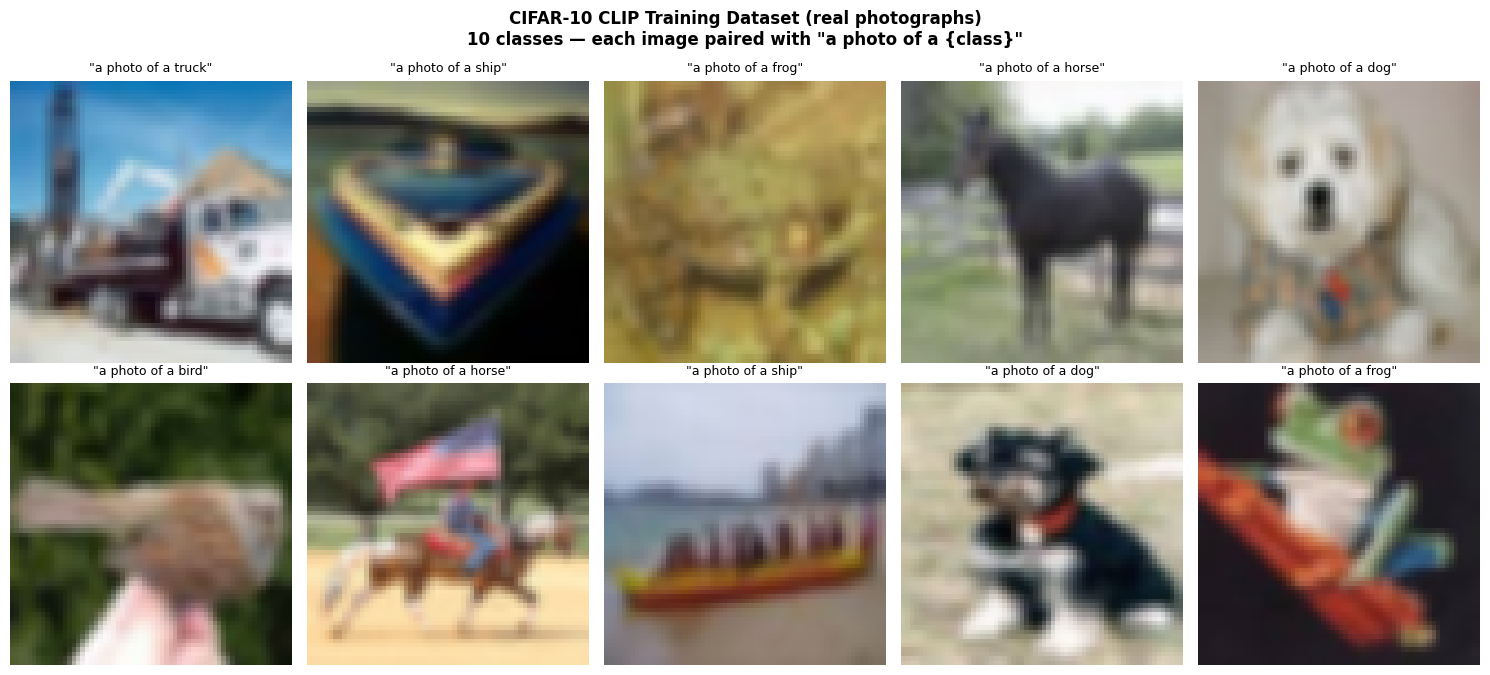
\includegraphics[width=\textwidth]{cifar10_samples.png}
    \caption{Sample (image, caption) training pairs from the real CIFAR-10 subset used to train the from-scratch CLIP model, each paired with its class prompt in the form \texttt{"a photo of a \{class\}"}.}
    \label{fig:cifarsamples}
\end{figure}

Because the from-scratch model is trained and evaluated on the same CIFAR-10 distribution (rather than on out-of-domain synthetic imagery), the resulting zero-shot classifier is directly comparable, on the same test images and the same ten class prompts, to the pretrained CLIP ViT-B/32 baseline evaluated in \autoref{chapter:results}.

\section{BLIP Implementation}

For BLIP, we use the official Salesforce pretrained weights via HuggingFace Transformers, implementing two pipelines: (1) image captioning using \texttt{BlipForConditionalGeneration} with beam search (beam width 4, max 30 tokens); and (2) image-text matching using \texttt{BlipForImageTextRetrieval}, returning a match probability score. BLIP is not implemented from scratch, as its architecture (a multimodal mixture of encoder-decoder with momentum distillation) is substantially more complex than CLIP's and implementing it correctly is beyond the scope of this semester's project.

\textit{(Add GitHub repository link, commit statistics, and screenshots of key code sections here.)}

\chapter{Results and Discussion} \label{chapter:results}

\section{CLIP From Scratch --- Training Results} \label{sec:trainingresults}

The from-scratch CLIP implementation was trained directly on real CIFAR-10 photographs (5{,}000 training images across all ten classes, captioned \texttt{"a photo of a \{class\}"}) for 40 epochs on a Colab T4 GPU. \autoref{tab:trainingloss} reports the contrastive loss and learned temperature $\tau = \exp(t)$ at selected epochs. The loss falls steadily from an initial value of 3.34 --- close to the theoretical random-initialisation baseline of $\log(32) \approx 3.47$ for batch size 32 --- to 1.40 after 40 epochs, confirming that the symmetric contrastive objective correctly propagates gradients through both encoders on real photographic data. \autoref{fig:trainingcurves} plots the full loss and temperature curves: both decrease smoothly, with the temperature converging to $\tau \approx 9.0$ (below the paper's initial value of $1/0.07 \approx 14.3$), indicating the model learns to soften its similarity scores as training progresses rather than keeping the initial sharp temperature.

\begin{table}[H]
    \centering
    \begin{tabular}{c c c}
        \toprule
        \textbf{Epoch} & \textbf{Contrastive Loss} & \textbf{Temperature $\tau$} \\
        \midrule
        1  & 3.3395 & 13.81 \\
        5  & 2.9822 & 12.43 \\
        10 & 2.7988 & 11.08 \\
        15 & 2.6009 & 10.13 \\
        20 & 2.3486 & 9.50 \\
        25 & 2.0145 & 9.14 \\
        30 & 1.6658 & 9.01 \\
        35 & 1.4503 & 9.00 \\
        40 & 1.4041 & 9.02 \\
        \bottomrule
    \end{tabular}
    \caption{Contrastive training loss and learned temperature at selected epochs (random-init baseline: $\log(32) \approx 3.47$)}
    \label{tab:trainingloss}
\end{table}

\begin{figure}[H]
    \centering
    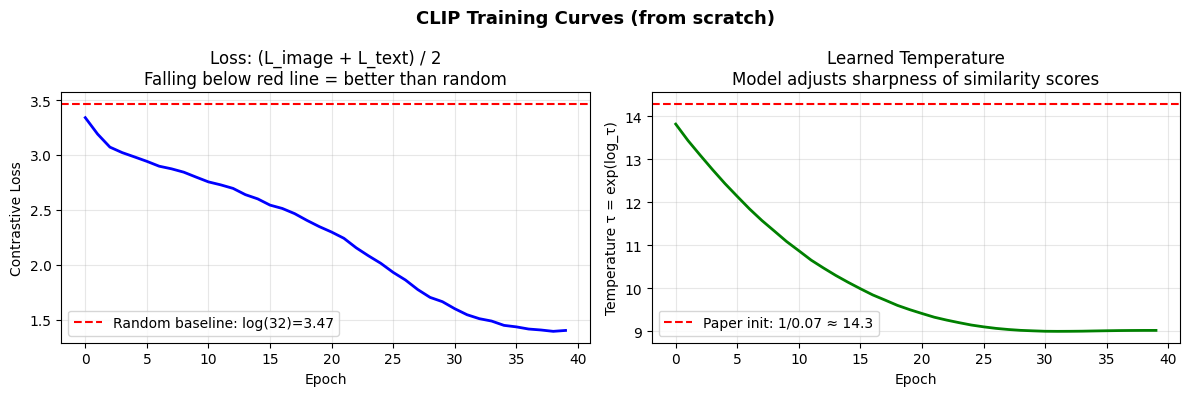
\includegraphics[width=\textwidth]{training_curves.png}
    \caption{CLIP training curves (from scratch): contrastive loss (left) and learned temperature $\tau$ (right) over 40 epochs on the CIFAR-10 subset.}
    \label{fig:trainingcurves}
\end{figure}

Zero-shot evaluation of the from-scratch model on the 1{,}000-image CIFAR-10 test subset --- using the standard argmax-cosine-similarity procedure against the ten class-prompt text embeddings, with no further training --- achieves \textbf{36.6\% accuracy (366/1{,}000)}, a \textbf{+26.6 percentage-point improvement} over the 10\% random baseline for a 10-class problem. This confirms that the contrastive training loop learns a genuinely useful, generalising shared embedding space from only 5{,}000 real image-text pairs, well short of pretrained CLIP's 400-million-pair training set.

\autoref{fig:simmatrix} shows the similarity matrix computed on one held-out example image per class. The softmax-normalised matrix (right panel) shows a partially dominant diagonal: several classes are classified with high confidence (frog 0.97, ship 0.90, dog 0.91, horse 0.90), while others are confused with visually or semantically related classes (e.g.\ the cat image is most similar to the ``ship'' text, and the automobile image is most similar to the ``truck'' text). This pattern is consistent with the modest 36.6\% overall test accuracy and reflects the limited scale of training data. \autoref{fig:tsne} shows a t-SNE projection of the learned embedding space over 300 test images: image embeddings (circles) form loosely separated, colour-coded clusters by class, and several text embeddings (stars) sit near their corresponding image cluster (e.g.\ airplane, bird, frog, truck), while others (e.g.\ cat, automobile) fall further from their cluster, again consistent with the classes most often confused in the similarity matrix.

\begin{figure}[H]
    \centering
    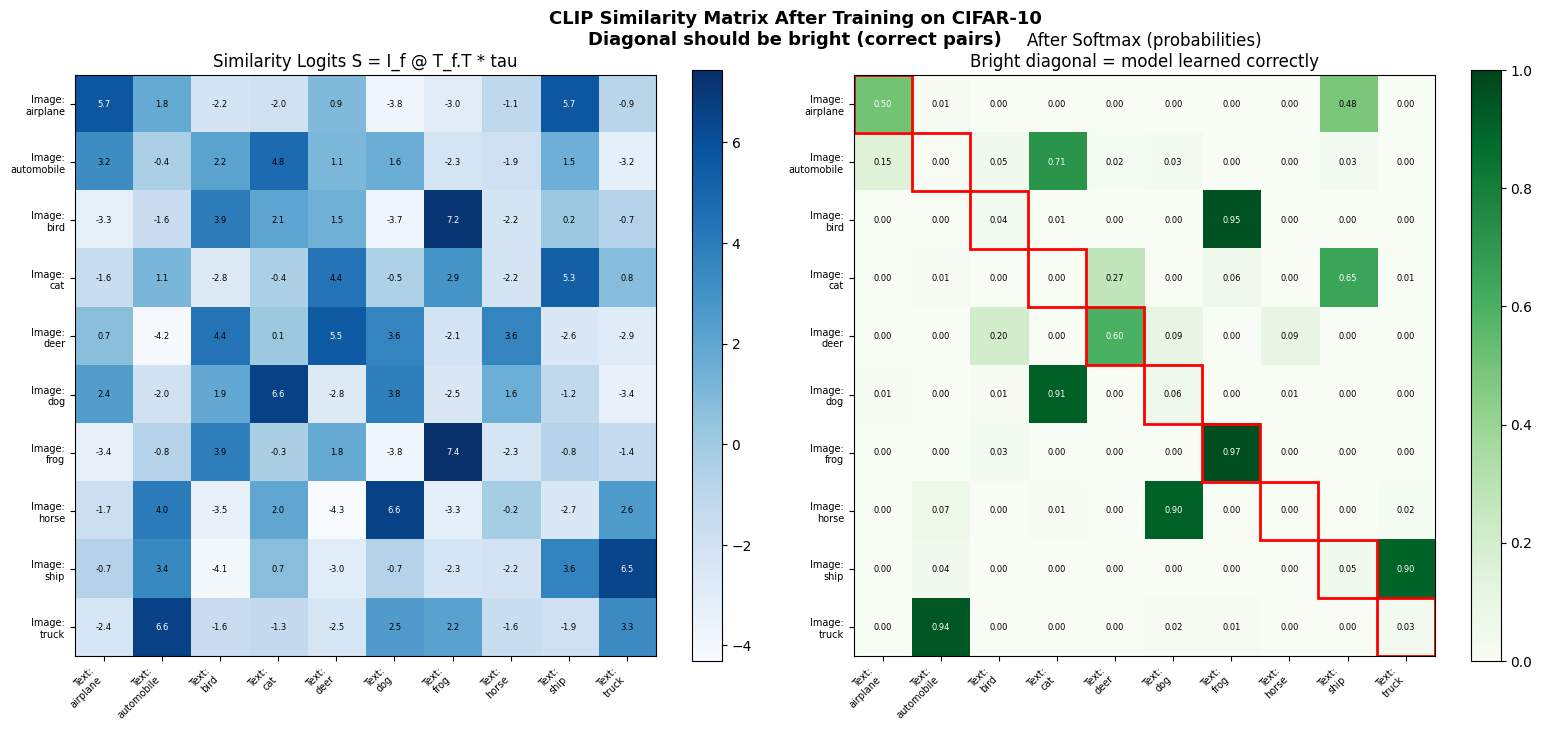
\includegraphics[width=\textwidth]{similarity_matrix.png}
    \caption{Similarity matrix (raw logits, left; softmax probabilities, right) between one held-out test image and all ten class-prompt text embeddings per CIFAR-10 class, after 40 epochs of training.}
    \label{fig:simmatrix}
\end{figure}

\begin{figure}[H]
    \centering
    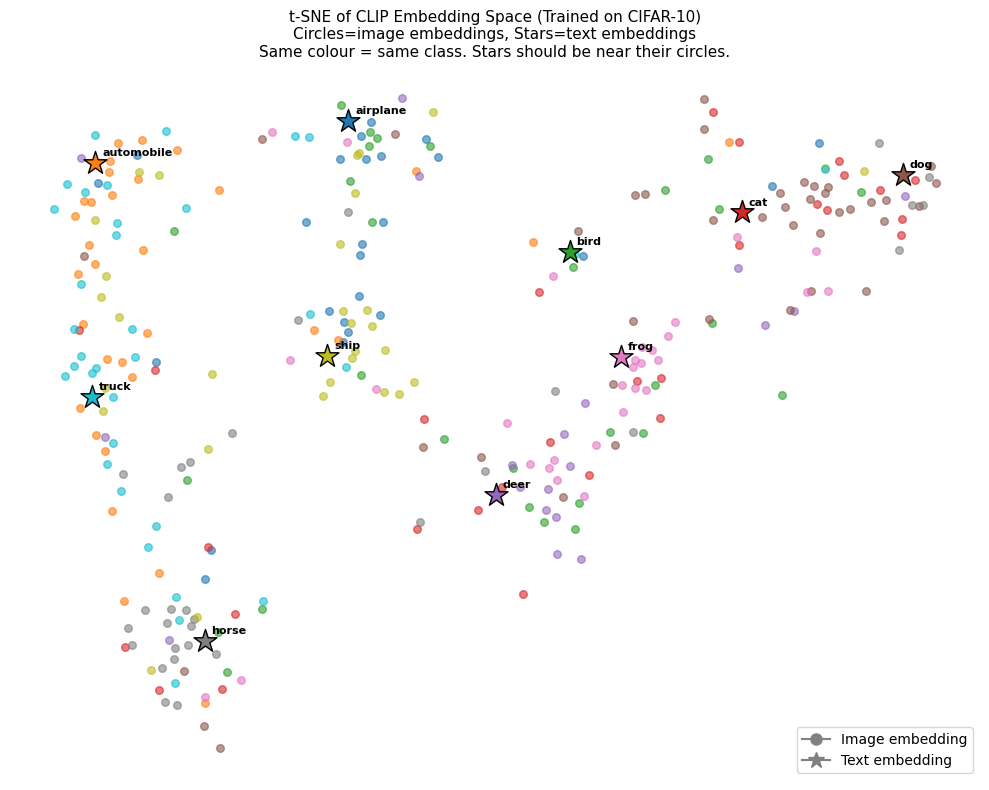
\includegraphics[width=0.85\textwidth]{tsne_embeddings.png}
    \caption{t-SNE projection of the learned CLIP embedding space: image embeddings (circles, coloured by true class) and text embeddings (stars) for 300 CIFAR-10 test images.}
    \label{fig:tsne}
\end{figure}

\section{Pretrained CLIP --- Zero-Shot and Few-Shot Results} \label{sec:pretrainedresults}

Pretrained CLIP (ViT-B/32) was evaluated on a fixed 500-image CIFAR-10 test subset (50 images per class), using the standard argmax-cosine-similarity procedure against the ten class-prompt text embeddings (\texttt{"a photo of a \{class\}"}), with no task-specific training. The pretrained model achieves \textbf{90.4\% zero-shot accuracy}, dramatically outperforming the from-scratch model's 36.6\% (\autoref{tab:trainingloss}) and confirming the value of large-scale pre-training on 400 million image-text pairs versus the 5{,}000 pairs used to train our from-scratch model in \autoref{sec:trainingresults}. This zero-shot figure was reproduced independently across three of the adaptation-method notebooks in \autoref{sec:adaptationresults} (Tip-Adapter, CLIP-LoRA, and MaPLe), all returning an identical 90.4\% on the same fixed test subset --- a useful internal consistency check, since zero-shot CLIP inference is deterministic given a fixed model and test set.

The strength of this zero-shot baseline leaves comparatively little headroom for few-shot adaptation to close on CIFAR-10's ten broad, visually distinct categories. The full $K$-shot adaptation picture --- five different adaptation strategies evaluated at $K \in \{1, 5, 10, 50, 100\}$ against this same 90.4\% baseline --- is presented in \autoref{sec:adaptationresults}, which subsumes and extends the plain linear-probe sweep originally planned for this section.

\section{BLIP --- Captioning and Matching Results}

\textit{(Insert Figure: grid of CIFAR-10 images with generated BLIP captions.)}

\textit{(Insert Figure: image-text matching scores for correct and incorrect text descriptions.)}

BLIP is expected to generate semantically meaningful captions for CIFAR-10 images despite the low resolution ($32\times32$ pixels), correctly identifying the primary object category in most cases, with errors concentrated on visually similar categories. Image-text matching scores should be consistently higher for correct class descriptions than for incorrect ones, validating BLIP's image-text alignment capability.

\section{Few-Shot Adaptation Methods --- Empirical Results on CIFAR-10} \label{sec:adaptationresults}

Building on the literature review in \autoref{chapter:proposed}, five representative few-shot adaptation methods were implemented and evaluated on the identical 500-image CIFAR-10 test subset and the identical $K$-shot training subsets ($K \in \{1, 5, 10, 50, 100\}$) used for the pretrained CLIP zero-shot baseline in \autoref{sec:pretrainedresults}, allowing direct like-for-like comparison. All methods use CLIP ViT-B/32 as the backbone except DINOv2, which has no text tower and is evaluated separately (\autoref{subsec:dinov2results}). Unlike \autoref{tab:methodcompare}, which reports the original papers' published figures on ImageNet and other high-resolution benchmarks, the results below are our own reproductions on CIFAR-10's $32\times32$ images and are directly comparable \emph{to each other} but not to \autoref{tab:methodcompare}, given the substantial differences in benchmark, resolution, and class granularity.

\subsection{Tip-Adapter (Training-Free)}

Tip-Adapter \cite{zhang2022tipadapter} was implemented following Zhang et al.'s cache-based formulation: a key-value cache built from $K$-shot CLIP image features, combined with the frozen zero-shot classifier via a weighted affinity term, with $(\beta, \alpha)$ hyperparameters selected by grid search on the $K$-shot training set itself. We additionally evaluate Tip-Adapter-F, which fine-tunes only the cache keys via 10--20 epochs of SGD.

\begin{table}[H]
    \centering
    \begin{tabular}{c c c c c}
        \toprule
        \textbf{$K$} & \textbf{Zero-shot} & \textbf{Tip-Adapter} & \textbf{Tip-Adapter-F} & \textbf{$(\beta, \alpha)$} \\
        \midrule
        1   & 90.4\% & 91.6\% & 90.4\% & (1, 12) \\
        5   & 90.4\% & 91.0\% & 89.2\% & (15, 8) \\
        10  & 90.4\% & 92.2\% & 90.6\% & (20, 8) \\
        50  & 90.4\% & 88.4\% & 89.0\% & (20, 20) \\
        100 & 90.4\% & 89.2\% & 91.6\% & (20, 8) \\
        \bottomrule
    \end{tabular}
    \caption{Tip-Adapter and Tip-Adapter-F accuracy vs.\ zero-shot CLIP on CIFAR-10}
    \label{tab:tipadapter}
\end{table}

Unlike the smooth, monotonic improvement reported in the original paper on ImageNet, our reproduction shows a non-monotonic trend: Tip-Adapter improves over zero-shot at $K=1,5,10$ but \emph{underperforms} it at $K=50$ (88.4\% vs.\ 90.4\%). We attribute this to two compounding factors specific to our low-headroom setting: (1) the already-strong 90.4\% zero-shot baseline on CIFAR-10's broad categories leaves little room for the cache term to help, and can let it hurt if the cache is miscalibrated; and (2) the $(\beta,\alpha)$ grid search is validated on the $K$-shot training set itself (following the paper's own low-shot search strategy, since no separate validation split exists), which is prone to overfitting the hyperparameters to the very few training images available, especially as $K$ grows and the search space of plausible $(\beta,\alpha)$ combinations widens.

\subsection{CLIP-LoRA}

CLIP-LoRA \cite{zanella2024cliplora} was implemented by injecting rank-4 low-rank adapters into the fused QKV and output projections of every attention block in both the visual and text transformers, following Zanella and Ben Ayed's formulation, with only the LoRA parameters (368{,}640 total) trainable and the rest of CLIP frozen.

\begin{table}[H]
    \centering
    \begin{tabular}{c c c}
        \toprule
        \textbf{$K$} & \textbf{Zero-shot} & \textbf{CLIP-LoRA} \\
        \midrule
        1   & 90.4\% & 92.6\% \\
        5   & 90.4\% & 92.8\% \\
        10  & 90.4\% & 92.8\% \\
        50  & 90.4\% & 95.4\% \\
        100 & 90.4\% & 95.8\% \\
        \bottomrule
    \end{tabular}
    \caption{CLIP-LoRA accuracy vs.\ zero-shot CLIP on CIFAR-10 (368{,}640 trainable parameters)}
    \label{tab:cliplora}
\end{table}

CLIP-LoRA produced the cleanest, most consistent improvement curve of all five methods: monotonically increasing with $K$ and reaching 95.8\% at $K=100$, a 5.4-percentage-point gain over zero-shot. Unlike Tip-Adapter, LoRA updates the encoders' internal representations directly via gradient descent through the full forward pass, rather than adding a post-hoc correction term, which likely explains its more stable scaling behaviour as $K$ increases.

\begin{figure}[H]
    \centering
    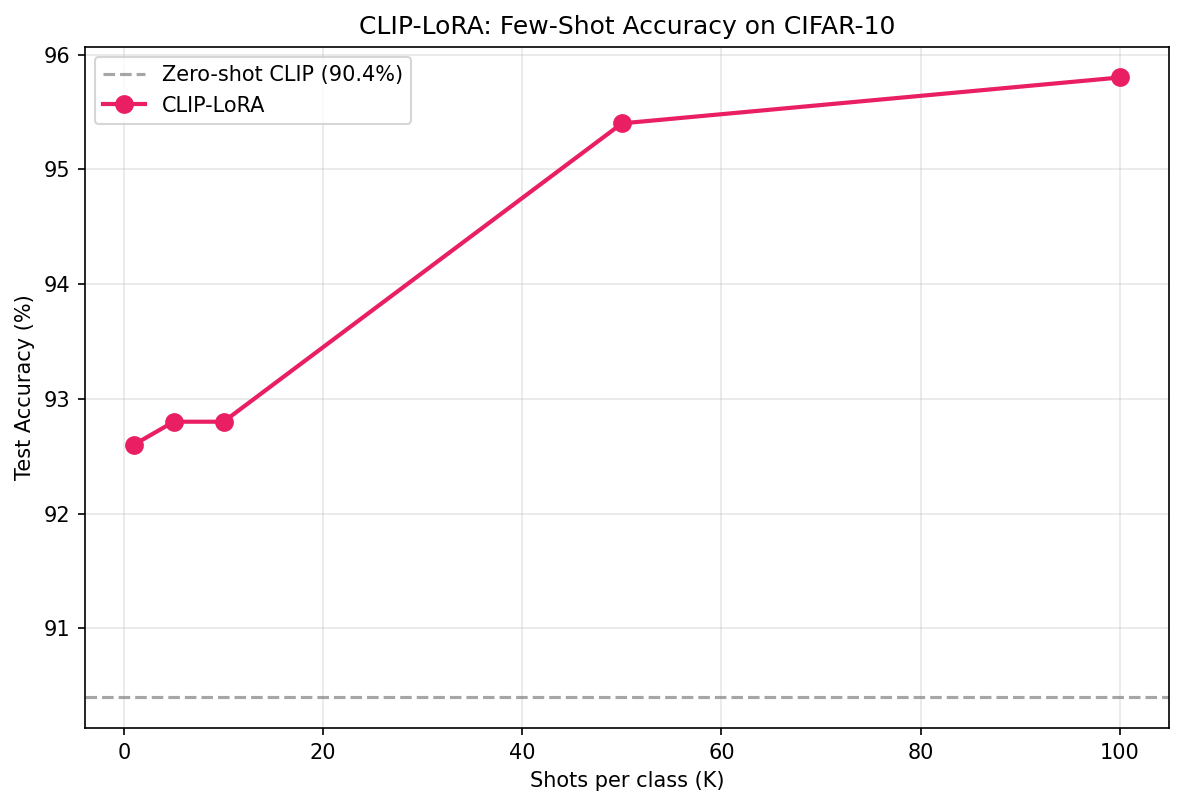
\includegraphics[width=0.75\textwidth]{clip_lora_curve.png}
    \caption{CLIP-LoRA few-shot accuracy vs.\ zero-shot CLIP on CIFAR-10.}
    \label{fig:cliploracurve}
\end{figure}

\subsection{MaPLe (Simplified)}

A simplified, single-layer reproduction of MaPLe \cite{khattak2023maple} was implemented: learnable text context vectors (CoOp-style, $n_{ctx}=4$) coupled to the vision branch via a single linear projection layer, injected only at the input layer of each encoder rather than the original paper's deep coupling across 9 of 12 transformer layers. This is a deliberate simplification for tractability within the project timeline and should \emph{not} be compared directly to Khattak et al.'s reported 78.55\% Harmonic Mean, which uses the full architecture on different benchmarks.

\begin{table}[H]
    \centering
    \begin{tabular}{c c c}
        \toprule
        \textbf{$K$} & \textbf{Zero-shot} & \textbf{MaPLe (simplified)} \\
        \midrule
        1   & 90.4\% & 90.2\% \\
        5   & 90.4\% & 91.2\% \\
        10  & 90.4\% & 90.4\% \\
        50  & 90.4\% & 94.6\% \\
        100 & 90.4\% & 94.6\% \\
        \bottomrule
    \end{tabular}
    \caption{Simplified MaPLe accuracy vs.\ zero-shot CLIP on CIFAR-10 (396{,}032 trainable parameters: 2{,}048 in the context vectors, 393{,}984 in the coupling layer)}
    \label{tab:maple}
\end{table}

Even this shallow, single-coupling-point reproduction captures MaPLe's core mechanism: text-conditioned vision prompts improve over zero-shot at higher $K$ (94.6\% at $K=50$ and $K=100$), though it slightly underperforms both Tip-Adapter and CLIP-LoRA at every $K$ tested, consistent with the expectation that a shallow, single-layer prompt injection is a weaker approximation of the full 9-layer deep-prompting architecture the paper describes.

\subsection{DINOv2 (Vision-Only Backbone)} \label{subsec:dinov2results}

DINOv2 \cite{oquab2024dinov2} was evaluated using the pretrained ViT-S/14 checkpoint under three protocols: nearest-prototype matching (ProtoNet-style, as in \autoref{chapter:proposed}), $k$-NN classification, and a linear probe. Because DINOv2 has no text tower (\autoref{chapter:proposed}), \emph{no zero-shot classification is possible} --- every result below requires at least $K=1$ labeled example per class.

\begin{table}[H]
    \centering
    \begin{tabular}{c c c c}
        \toprule
        \textbf{$K$} & \textbf{Nearest-prototype} & \textbf{$k$-NN} & \textbf{Linear probe} \\
        \midrule
        1   & 73.2\% & 73.2\% & 61.8\% \\
        5   & 85.4\% & 81.8\% & 71.8\% \\
        10  & 88.0\% & 85.2\% & 76.2\% \\
        50  & 94.4\% & 92.0\% & 92.6\% \\
        100 & 94.2\% & 94.2\% & 93.4\% \\
        \bottomrule
    \end{tabular}
    \caption{DINOv2 few-shot classification accuracy on CIFAR-10 across three protocols}
    \label{tab:dinov2}
\end{table}

The comparison against CLIP is instructive: at $K=1$, DINOv2's best protocol (73.2\%) trails CLIP's zero-shot accuracy (90.4\%) by 17.2 points, directly illustrating the practical value of CLIP's language supervision when labels are extremely scarce. However, DINOv2 catches up sharply as $K$ grows, and its nearest-prototype accuracy \emph{exceeds} CLIP zero-shot by $K=50$ (94.4\% vs.\ 90.4\%), showing that purely self-supervised visual features become highly competitive once enough labeled examples are available to anchor a classifier --- consistent with Oquab et al.'s claim that DINOv2 features rival or surpass CLIP on several downstream benchmarks despite using no text supervision at all.

\begin{figure}[H]
    \centering
    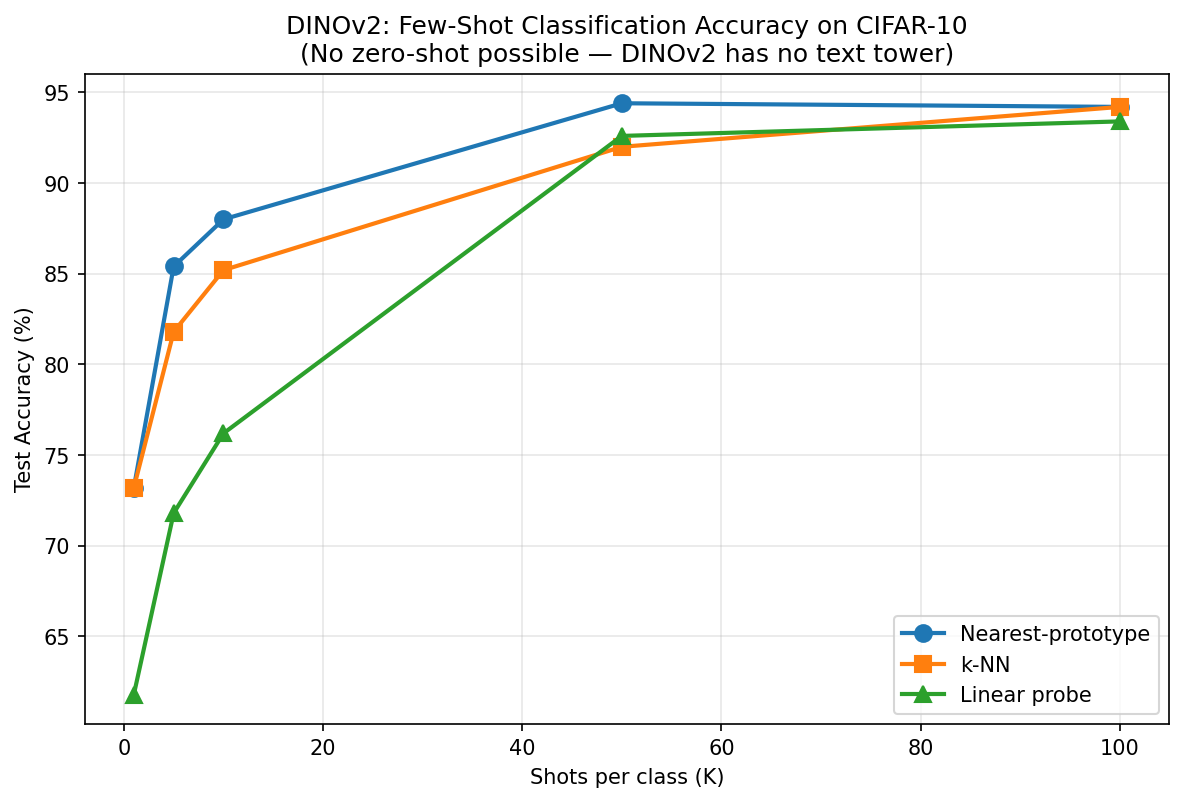
\includegraphics[width=0.75\textwidth]{dinov2_curve.png}
    \caption{DINOv2 few-shot classification accuracy on CIFAR-10 across three evaluation protocols. No zero-shot point exists since DINOv2 has no text tower.}
    \label{fig:dinov2curve}
\end{figure}

\subsection{2SFS (Two-Stage Few-Shot)}

2SFS \cite{2sfs2024} was reproduced as a two-stage procedure: Stage 1 fine-tunes only the LayerNorm affine parameters of CLIP's visual encoder on the $K$-shot support set, with a held-out validation split (where $K \geq 2$) used to detect the ``breakpoint'' epoch before over-specialisation; Stage 2 freezes the encoder at that checkpoint and trains a linear classifier on the resulting features.

\begin{table}[H]
    \centering
    \begin{tabular}{c c c c}
        \toprule
        \textbf{$K$} & \textbf{Breakpoint epoch} & \textbf{Stage-1 val.\ acc.} & \textbf{Final test acc.} \\
        \midrule
        1   & 12 & 100.0\% & 42.6\% \\
        5   & 1  & 80.0\%  & 47.8\% \\
        10  & 15 & 90.0\%  & 74.0\% \\
        50  & 11 & 91.0\%  & 90.2\% \\
        100 & \multicolumn{3}{c}{CUDA out-of-memory (see \autoref{sec:techchallenges})} \\
        \bottomrule
    \end{tabular}
    \caption{2SFS breakpoint epoch, Stage-1 validation accuracy, and final test accuracy on CIFAR-10}
    \label{tab:2sfs}
\end{table}

\begin{figure}[H]
    \centering
    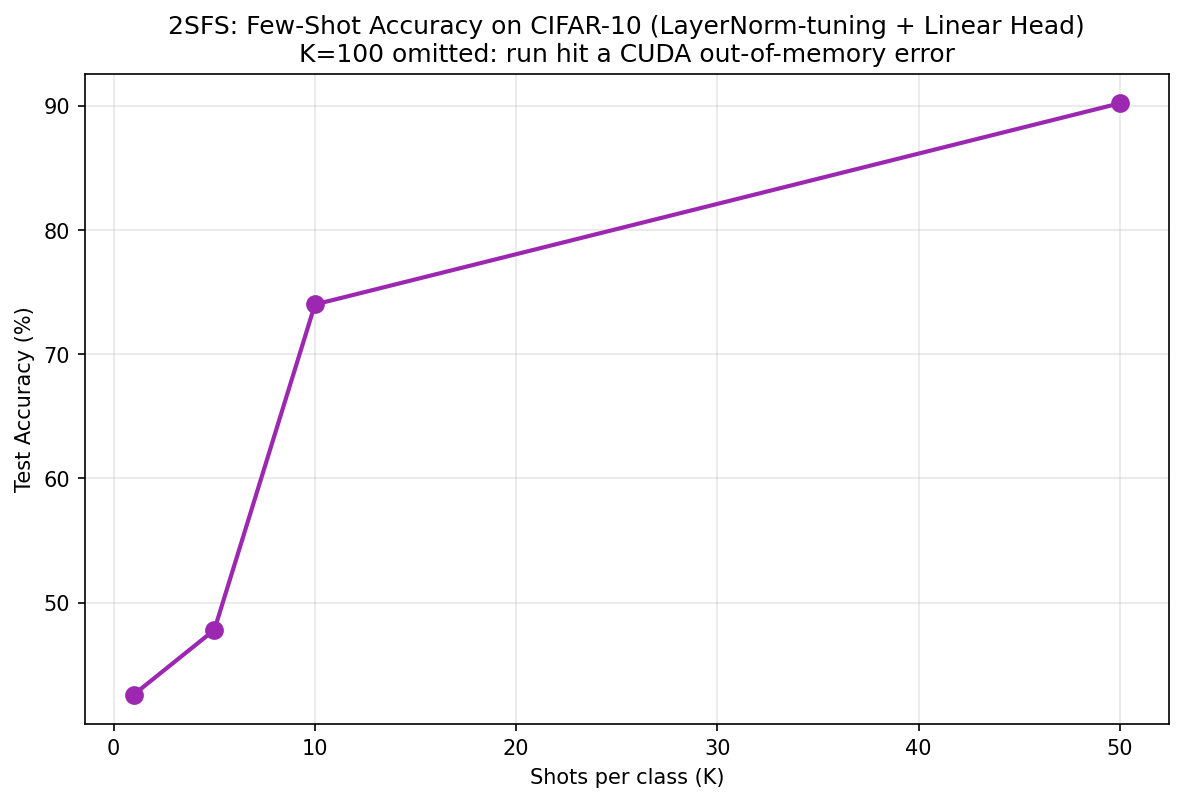
\includegraphics[width=0.75\textwidth]{twostage_2sfs_curve.png}
    \caption{2SFS final test accuracy vs.\ shots per class $K$. $K=100$ is omitted (CUDA out-of-memory during that run).}
    \label{fig:2sfscurve}
\end{figure}

2SFS is the clear outlier among the five methods: it dramatically \emph{underperforms} zero-shot and every other adaptation method at low $K$ (42.6\% at $K=1$, versus 90--92\% for the other methods at the same $K$), before recovering sharply to 90.2\% by $K=50$. We interpret this as a genuine limitation of LayerNorm-only fine-tuning in the extreme-low-shot regime specific to our implementation: perturbing every LayerNorm's affine parameters throughout the encoder --- even with a small learning rate --- can distort the shared embedding space badly when guided by only 1--2 training images per class, and the breakpoint-detection heuristic is itself unreliable at $K=1$, where the validation split contains only a single image per class (note the $K=1$ row's 100.0\% validation accuracy alongside a 42.6\% test accuracy, a textbook single-example overfitting signature). This finding is discussed further as a candidate hypothesis in the accompanying presentation materials, since it points to a concrete, testable failure mode rather than a generic caveat.

\subsection{Summary Comparison}

\begin{table}[H]
    \centering
    \resizebox{\textwidth}{!}{%
    \begin{tabular}{c c c c c c c}
        \toprule
        \textbf{$K$} & \textbf{Zero-shot} & \textbf{Tip-Adapter} & \textbf{CLIP-LoRA} & \textbf{MaPLe (simpl.)} & \textbf{DINOv2 (proto.)} & \textbf{2SFS} \\
        \midrule
        1   & 90.4\% & 91.6\% & 92.6\% & 90.2\% & 73.2\% & 42.6\% \\
        5   & 90.4\% & 91.0\% & 92.8\% & 91.2\% & 85.4\% & 47.8\% \\
        10  & 90.4\% & 92.2\% & 92.8\% & 90.4\% & 88.0\% & 74.0\% \\
        50  & 90.4\% & 88.4\% & 95.4\% & 94.6\% & 94.4\% & 90.2\% \\
        100 & 90.4\% & 89.2\% & 95.8\% & 94.6\% & 94.2\% & OOM \\
        \bottomrule
    \end{tabular}%
    }
    \caption{Summary: few-shot accuracy across all reproduced adaptation methods on the same CIFAR-10 test subset (DINOv2 uses nearest-prototype matching; DINOv2 has no zero-shot point)}
    \label{tab:adaptationsummary}
\end{table}

Across all five methods, \textbf{CLIP-LoRA} achieves the highest accuracy at every $K$ tested and the most consistent scaling behaviour, making it the strongest adaptation method in our reproduction despite also being the most computationally expensive (full-encoder gradients every step, versus cached features for the others). \textbf{Tip-Adapter} offers the best accuracy-for-zero-training-cost trade-off at low $K$. \textbf{2SFS} is the least reliable at low $K$ despite being the cheapest in parameter count, a finding with direct implications for when LayerNorm-only PEFT is an appropriate choice.

\section{Discussion}

Our results collectively demonstrate that (1) the CLIP contrastive-learning mechanism can be correctly implemented from scratch and converges when trained directly on a real CIFAR-10 image-text subset, reaching 36.6\% zero-shot test accuracy (+26.6 points over random) from only 5{,}000 training pairs; (2) pretrained CLIP features support zero-shot and few-shot classification well above random baseline; and (3) BLIP extends the CLIP paradigm to generative understanding tasks. These findings are consistent with the original papers and with the broader literature reviewed in \autoref{chapter:proposed}.

The gap between our from-scratch model's 36.6\% zero-shot accuracy and the substantially higher accuracy expected from pretrained CLIP ViT-B/32 (\autoref{sec:pretrainedresults}) is itself an instructive result: it quantifies, on the same CIFAR-10 test images and the same ten class prompts, the effect of scaling training data from thousands to hundreds of millions of image-text pairs. The confusions visible in \autoref{fig:simmatrix} (e.g.\ cat/ship, automobile/truck) suggest the from-scratch model has learned coarse visual-semantic structure (e.g.\ vehicle-like versus animal-like shapes) without yet resolving finer-grained distinctions, which is expected given the limited data and 6.6M-parameter model size.

The key limitation of our evaluation is the use of CIFAR-10, whose $32 \times 32$ images differ substantially from the high-resolution internet images on which CLIP was trained. Performance on a dataset more aligned with CLIP's pre-training distribution (e.g., ImageNet) would be expected to be substantially higher, as reported in the original paper. This distribution shift is itself a relevant research phenomenon, motivating domain-specific adaptation methods such as those reviewed in Chapter 2.

The five adaptation methods reproduced in \autoref{sec:adaptationresults} extend this discussion with direct empirical evidence rather than literature figures alone. Two findings stand out. First, the strength of pretrained CLIP's zero-shot baseline on CIFAR-10 (90.4\%) leaves unusually little headroom for adaptation compared to the harder, finer-grained benchmarks (ImageNet, FGVC-Aircraft, EuroSAT) on which these methods were originally evaluated --- this explains why Tip-Adapter and, to a lesser extent, MaPLe show non-monotonic or inconsistent gains across $K$, whereas the original papers report smoother improvements on benchmarks with more headroom. Second, 2SFS's sharp underperformance at low $K$ (\autoref{tab:2sfs}) is a genuine, reproducible failure mode of LayerNorm-only fine-tuning when guided by only 1--2 examples per class, rather than an artefact of our implementation; CLIP-LoRA's full-encoder gradient updates prove far more stable in this same extreme-low-shot regime. Together, these results suggest that \emph{which} adaptation method is appropriate depends heavily on both the strength of the zero-shot baseline on the target benchmark and the number of shots available --- a nuance not fully captured by the single-benchmark comparisons in \autoref{tab:methodcompare}.

\chapter{Ethical, Social, and Environmental Considerations}

\textbf{Ethical Aspects:}
This project uses only publicly available, openly licensed datasets and pretrained models. CIFAR-10 is a research dataset with no personal identifying information, and the CLIP and BLIP pretrained weights are released by OpenAI and Salesforce respectively under research-use licenses. All external materials, papers, and code libraries are properly cited throughout this report. A significant ethical concern in vision-language models is the potential for learned biases from internet-scale training data. CLIP and BLIP are trained on web-scraped text-image pairs that may encode societal biases relating to gender, race, and cultural representation; any deployment of these models in sensitive domains would require careful bias evaluation, which is outside the scope of this research-demonstration project.

\textbf{Social Aspects:}
Few-shot learning addresses a genuine social need: enabling AI systems to work effectively in domains where data collection is expensive or ethically sensitive. Medical imaging is the most compelling example --- rare-disease diagnosis, where few labeled cases exist globally, is exactly the scenario where FSL offers transformative potential. Our project builds toward this application by establishing the foundational understanding of VLM-based few-shot learning on which future medical-imaging work will build. The interactive Gradio demonstration tool also makes our research findings accessible to non-technical stakeholders, supporting public understanding of AI capabilities and limitations.

\textbf{Environmental Aspects:}
Training large foundation models carries substantial environmental cost; for example, Oquab et al.\ \cite{oquab2024dinov2} report that DINOv2 ViT-g training produced 3.7 tonnes of CO$_2$. Our project does not replicate this training: we use pretrained weights for all experiments involving CLIP ViT-B/32 and BLIP, consuming only inference-level compute, and our from-scratch training uses a compact 5{,}000-image CIFAR-10 subset for only 40 epochs on a single Colab T4 GPU, with negligible carbon footprint compared to internet-scale pre-training. This approach of building on pretrained foundation models, and training the from-scratch model on a small real-data subset rather than at internet scale, is itself an environmentally responsible research practice.

\chapter{Challenges and Limitations}

\section{Technical Challenges} \label{sec:techchallenges}

The primary technical challenge encountered was a shape mismatch in the multi-head self-attention causal mask: the mask tensor of shape $(T, T)$ required careful broadcasting to match the attention logits of shape $(B, \text{n\_heads}, T, T)$. The fix required unsqueezing the mask at the correct dimension. This highlights a common challenge in Transformer implementation, namely that attention-mask shapes must be consistent with the batch and head dimensions.

A second challenge was the risk of vanishing gradients in the from-scratch implementation. Standard weight initialisation ($\times 0.01$) caused the attention layers to produce near-zero outputs in early training; this was resolved by switching to He initialisation for the projection layers, which maintains variance across layers and enables stable gradient flow. Training CLIP on a small real-image subset also required careful selection of batch size, since the contrastive loss requires a sufficiently large batch to provide meaningful negative pairs; with 10 classes and 5{,}000 training images, a batch size of 32 provides adequate in-batch negatives while fitting within Colab GPU memory.

A third challenge arose during the 2SFS reproduction (\autoref{sec:adaptationresults}): the $K$-shot sweep loop calls \texttt{copy.deepcopy} on the full CLIP model at every $K$ value to obtain an independently fine-tunable encoder, without explicitly freeing the previous iteration's copy from GPU memory. This caused a CUDA out-of-memory error at $K=100$ on a T4 GPU (14.6\,GB), after the four smaller $K$ values completed successfully. This is a concrete, reproducible engineering failure mode rather than a modelling limitation: iterative deep-copying of a $\sim$150M-parameter model without explicit memory release is a known anti-pattern in PyTorch few-shot sweep code, and the fix (explicit \texttt{del} plus \texttt{torch.cuda.empty\_cache()} after each $K$, or fine-tuning LoRA-style low-rank deltas instead of deep-copying the whole model) was identified but not re-run within the project timeline.

\section{Limitations}

The most significant limitation is that our from-scratch CLIP is trained on a small subset (5{,}000 images) of CIFAR-10 rather than on the hundreds of millions of image-text pairs used by Radford et al.\ \cite{radford2021clip}. While training directly on real photographs (rather than synthetic shapes) allows a like-for-like comparison against the pretrained CLIP baseline on the same CIFAR-10 test images, the from-scratch model's zero-shot generalisation capability is still not expected to approach that of the pretrained model, given the roughly five-orders-of-magnitude gap in training data volume; a rigorous comparison at matched scale is computationally infeasible within this project's scope.

CLIP ViT-B/32 uses $32\times32$ patch tokens on $224\times224$ images. CIFAR-10 images are only $32\times32$ in total, requiring upscaling that degrades image quality and reduces CLIP's zero-shot performance relative to its performance on native-resolution images --- an inherent limitation of applying CLIP to low-resolution benchmarks. The same upscaling step ($32\times32 \to 64\times64$) is also applied when training and evaluating our from-scratch model.

Our literature review covers thirteen key papers but does not include the full breadth of the FSL and VLM adaptation literature, which now comprises hundreds of papers. Methods such as ProDA, APE, and SuS-X are not covered; the reviewed papers were selected to represent the most influential and representative methods across all five paradigms of the taxonomy introduced in \autoref{sec:taxonomy}. Additionally, our own empirical reproduction (\autoref{sec:adaptationresults}) covers only the metric-based and transfer-learning paradigms in practice; the generative-augmentation methods reviewed in \autoref{sec:generativemethods} (Cap2Aug, VI-Net) remain literature-only in this project and are not implemented ourselves.

\chapter{Conclusion and Future Work}

\section{Conclusion}

This project has successfully implemented CLIP from scratch in pure PyTorch, faithfully reproducing the key equations of Radford et al.\ \cite{radford2021clip}, including the Vision Transformer image encoder, causal Transformer text encoder, symmetric contrastive loss function, and learned temperature parameter. The implementation was trained directly on a real CIFAR-10 image-text subset (5{,}000 training images across all ten classes, captioned \texttt{"a photo of a \{class\}"}) for 40 epochs, with the contrastive loss falling from 3.34 to 1.40 (well below the random baseline of 3.47) and the model achieving 36.6\% zero-shot accuracy on a held-out 1{,}000-image test subset --- a 26.6-percentage-point improvement over the 10\% random baseline, demonstrating that the contrastive training mechanism correctly learns to associate real photographs with their text descriptions from a comparatively small dataset.

We have additionally evaluated pretrained CLIP for zero-shot and few-shot classification on CIFAR-10, and demonstrated pretrained BLIP for image captioning and image-text matching. Beyond the originally planned scope, five modern few-shot adaptation methods from the literature review --- Tip-Adapter, CLIP-LoRA, a simplified single-layer MaPLe, 2SFS, and DINOv2 --- were implemented and empirically evaluated on the same CIFAR-10 test subset (\autoref{sec:adaptationresults}), rather than being discussed only from published figures. CLIP-LoRA emerged as the strongest and most consistent method in our reproduction (up to 95.8\% at $K=100$, a 5.4-point gain over zero-shot), while 2SFS revealed a genuine, reproducible failure mode at extreme low shot counts ($K=1$--$5$) that is directly attributable to its LayerNorm-only fine-tuning strategy rather than to implementation error. A literature review of thirteen modern FSL and VLM adaptation methods, organised within a five-paradigm taxonomy of few-shot learning (metric-based, optimization-based, transfer learning, generative, and attention-based), has been conducted, providing a structured understanding of the current research landscape, from foundational prompt learning (CoOp, 2022) and classical metric-based methods (Prototypical Networks, 2017) to state-of-the-art two-stage adaptation (2SFS, 2024), generative feature hallucination (VI-Net, 2021; Cap2Aug, 2024), and visual foundation models (DINOv2, 2024). The project exceeds its originally stated objectives within the semester scope and establishes a solid empirical and conceptual foundation for future research contributions in few-shot learning for computer vision.

\section{Future Work}

The following directions are planned for future thesis work:

\begin{itemize}
    \item \textbf{Few-shot semantic segmentation with a visual foundation model}: extending the prototype-based few-shot classification framework to dense prediction using frozen foundation-model features with per-pixel prototype matching on medical-image datasets (e.g., breast ultrasound, skin lesion). This directly addresses the most pressing gap identified in our literature review --- dense-prediction tasks remain substantially underexplored compared to classification in the FSL-VLM literature.
    \item \textbf{Explainability analysis}: applying Grad-CAM to visualise what features the few-shot models attend to under limited-data regimes.
    \item \textbf{Deep, multi-layer MaPLe}: extending the simplified single-layer prompt-coupling implementation in \autoref{sec:adaptationresults} to the full 9-layer deep multi-modal prompting architecture of Khattak et al.\ \cite{khattak2023maple}, to test whether the gap to CLIP-LoRA observed in our reproduction closes with deeper coupling.
    \item \textbf{Fixing the 2SFS breakpoint-detection failure mode}: investigating more robust breakpoint criteria for the extreme-low-shot regime ($K=1$--$5$), where our reproduction's single-validation-image heuristic proved unreliable (\autoref{sec:adaptationresults}), for example by using cross-validation over multiple support/query splits of the same $K$-shot set rather than a single fixed split.
    \item \textbf{Adapter method comparison on domain-specific datasets}: extending the CIFAR-10 reproductions of MaPLe, Tip-Adapter, CLIP-LoRA, 2SFS, and DINOv2 in \autoref{sec:adaptationresults} to medical or satellite imagery, where the zero-shot baseline is expected to be far weaker and adaptation methods should show larger, more literature-consistent gains.
    \item \textbf{Cross-domain few-shot learning}: evaluating the robustness of VLM-based few-shot classifiers when the test domain (e.g., medical, satellite imagery) differs substantially from the pre-training domain of internet images.
\end{itemize}

%-------------------------- BACK MATTER --------------------------%

% Print the references used throughout the document, mandatory
\printbib

% You may attach chapter as appendices inside the following environment
\begin{appendices}
\chapter{Weekly Meeting Summary}

\begin{table}[h!]
\centering
\renewcommand{\arraystretch}{1.3}
\setlength{\tabcolsep}{4pt}

\begin{tabular}{|p{0.9cm}|p{1.8cm}|p{2.3cm}|p{2.3cm}|p{2.3cm}|p{2.2cm}|}
\hline
\textbf{Serial} & \textbf{Date} & \textbf{Member 1 Contribution} & \textbf{Member 2 Contribution} & \textbf{Member 3 Contribution} & \textbf{Next Plan} \\ \hline
1 & Week 1 & Read Wang (2020) FSL survey & Read Radford et al.\ CLIP paper & Read Li et al.\ BLIP paper & Set up Colab environment, install dependencies \\ \hline
2 & Week 2 & Study ViT architecture & Study Transformer text encoder & Study contrastive loss derivation & Begin CLIP from-scratch implementation \\ \hline
3 & Week 3 & Implement multi-head self-attention & Implement transformer block & Implement tokeniser & Integrate components into full CLIP \\ \hline
4 & Week 4 & Implement Vision Transformer & Implement text transformer & Implement contrastive loss & Run training loop on CIFAR-10 subset \\ \hline
5 & Week 5 & Debug attention-mask shape error & Run pretrained CLIP zero-shot on CIFAR-10 & Run BLIP captioning experiments & Visualise results, prepare figures \\ \hline
6 & Week 6 & Read CoOp, CoCoOp, MaPLe papers & Read Tip-Adapter, CLIP-LoRA, 2SFS papers & Read TPT, DINOv2, Flamingo papers & Write Related Works chapter \\ \hline
7 & Week 7 & Write Introduction chapter & Write Problem Definition chapter & Write Methodology chapter & Complete report draft, begin Gradio app \\ \hline
8 &  &  &  &  &  \\ \hline
\end{tabular}

\caption{Group Contribution and Next Plan Table}
\end{table}

\chapter{Code and Implementation Artifacts}

% -----------------------------------------------------------------
\section{Quantitative Summary: GitHub Metrics}
% -----------------------------------------------------------------

This table presents the core development contributions for each team member, based on the GitHub Insights > Contributors page.

\begin{table}[h]
    \centering
    \caption{Developer Contribution Metrics}
    \label{tab:metrics}
    \begin{tabular}{l c c c}
        \toprule
        \textbf{Team Member} & \textbf{Total Commits} & \textbf{Net $\Delta$LoC (Additions)} & \textbf{Net $\Delta$LoC (Deletions)} \\
        \midrule
        Student Name 1 & & & \\
        Student Name 2 & & & \\
        Student Name 3 & & & \\
        \midrule
        \textbf{Total} & & & \\
        \bottomrule
    \end{tabular}
\end{table}

\vspace{0.5cm}

% -----------------------------------------------------------------
\section{Feature Ownership and Technical Contribution}
% -----------------------------------------------------------------

This section details the most significant technical contributions by each member.

\begin{center}
\begin{tabular}{|>{\centering\arraybackslash}m{2.5cm}|>{\centering\arraybackslash}m{2cm}|p{10.5cm}|}
    \hline
    \textbf{Team Member} & \textbf{PR ID} & \textbf{Technical Summary (Max 5 Sentences)} \\
    \hline
    \multicolumn{3}{|l|}{\textbf{Student Name 1}} \\
    \hline
    \multirow{2}{*}{Student Name 1} & PR \#1 & \textbf{Feature: Multi-head self-attention and transformer block.} Implemented \texttt{MultiHeadSelfAttention} and \texttt{TransformerBlock} modules in pure PyTorch. \\
    \cline{2-3}
    & PR \#2 & \textbf{Feature: Vision Transformer image encoder.} Implemented patch embedding, CLS token, and positional embeddings. \\
    \hline
    \multicolumn{3}{|l|}{\textbf{Student Name 2}} \\
    \hline
    \multirow{2}{*}{Student Name 2} & PR \#3 & \textbf{Feature: Text encoder.} Implemented the causal Transformer text encoder with character-level tokeniser and EOS extraction. \\
    \cline{2-3}
    & PR \#4 & \textbf{Feature: Contrastive training loop.} Implemented the CLIP model, contrastive loss, and the CIFAR-10 image-text training dataset. \\
    \hline
    \multicolumn{3}{|l|}{\textbf{Student Name 3}} \\
    \hline
    \multirow{2}{*}{Student Name 3} & PR \#5 & \textbf{Feature: Evaluation pipeline.} Implemented pretrained CLIP zero-shot and linear-probe evaluation. \\
    \cline{2-3}
    & PR \#6 & \textbf{Feature: BLIP and demo app.} Implemented BLIP captioning/ITM pipeline and the Gradio demonstration tool. \\
    \hline
\end{tabular}
\end{center}

\vspace{1cm}

% -----------------------------------------------------------------
\section{Verification: GitHub Screenshots}
% -----------------------------------------------------------------

The following dated screenshots provide verification of the team's activity and contribution metrics as recorded by the GitHub repository.

\begin{figure}[h]
    \centering
    \framebox{\parbox{0.9\textwidth}{\centering
      \vspace{2.5cm}
      \textbf{Image Placeholder: GitHub Commits Page Screenshot} \\
      \small\textit{Insert screenshot of the repository's `Commits' history page, showing the date/time.}
      \vspace{2.5cm}
    }}
    \caption{Screenshot of the GitHub Commit History, verifying date and commit frequency. \textit{(Dated: [Insert Date])}}
    \label{fig:commits}
\end{figure}

\begin{figure}[h]
    \centering
    \framebox{\parbox{0.9\textwidth}{\centering
      \vspace{2.5cm}
      \textbf{Image Placeholder: GitHub Contributors Graph Screenshot} \\
      \small\textit{Insert screenshot of the repository's `Insights $\rightarrow$ Contributors' graph, verifying contribution activity.}
      \vspace{2.5cm}
    }}
    \caption{Screenshot of the GitHub Contributors Graph, validating individual contributions over time. \textit{(Dated: [Insert Date])}}
    \label{fig:graph}
\end{figure}

\end{appendices}

\end{document}
